\let\negmedspace\undefined
\let\negthickspace\undefined
\documentclass[journal,12pt,onecolumn]{IEEEtran}
\usepackage{cite}
\usepackage{amsmath,amssymb,amsfonts,amsthm}
\usepackage{algorithmic}
\usepackage{graphicx}
\graphicspath{{./figs/}}
\usepackage{textcomp}
\usepackage{xcolor}
\usepackage{txfonts}
\usepackage{listings}
\usepackage{enumitem}
\usepackage{mathtools}
\usepackage{gensymb}
\usepackage{comment}
\usepackage{caption}
\usepackage[breaklinks=true]{hyperref}
\usepackage{tkz-euclide} 
\usepackage{listings}
\usepackage{gvv}                                        
%\def\inputGnumericTable{}                                 
\usepackage[latin1]{inputenc}     
\usepackage{xparse}
\usepackage{color}                                            
\usepackage{array}                                            
\usepackage{longtable}                                       
\usepackage{calc}                                             
\usepackage{multirow}
\usepackage{multicol}
\usepackage{hhline}                                           
\usepackage{ifthen}                                           
\usepackage{lscape}
\usepackage{tabularx}
\usepackage{array}
\usepackage{float}
\newtheorem{theorem}{Theorem}[section]
\newtheorem{problem}{Problem}
\newtheorem{proposition}{Proposition}[section]
\newtheorem{lemma}{Lemma}[section]
\newtheorem{corollary}[theorem]{Corollary}
\newtheorem{example}{Example}[section]
\newtheorem{definition}[problem]{Definition}
\newcommand{\BEQA}{\begin{eqnarray}}
\newcommand{\EEQA}{\end{eqnarray}}
\newcommand{\define}{\stackrel{\triangle}{=}}
\theoremstyle{remark}
\newtheorem{rem}{Remark}

\begin{document}
\title{
ASSIGNMENT 1: GATE EE 2025   \\
EC: ELECTRONICS AND COMMUNICATION ENGINEERING}
\author{AI25BTECH11019 - Sai Sanjana}
\maketitle
\renewcommand{\thefigure}{\theenumi}
\renewcommand{\thetable}{\theenumi}
\begin{enumerate}

\item If $ E $ denotes expectation, the variance of a random variable $ X $ is given by:
\hfill{\brak{\text{GATE EE 2025}}}
\begin{enumerate}
    
    \item $ E[X^2] - E^2[X] $
    \item $ E[X^2] + E^2[X] $
    \item $ E[X^2] $
    \item $ E^2[X] $

\end{enumerate}


\item The following plot shows a function $y$ which varies linearly with $x$. The value of the integral $\int_{0}^{2} y \, dx$ is:
\hfill{\brak{\text{GATE EE 2025}}}

\begin{figure}[ht!]
    \centering
    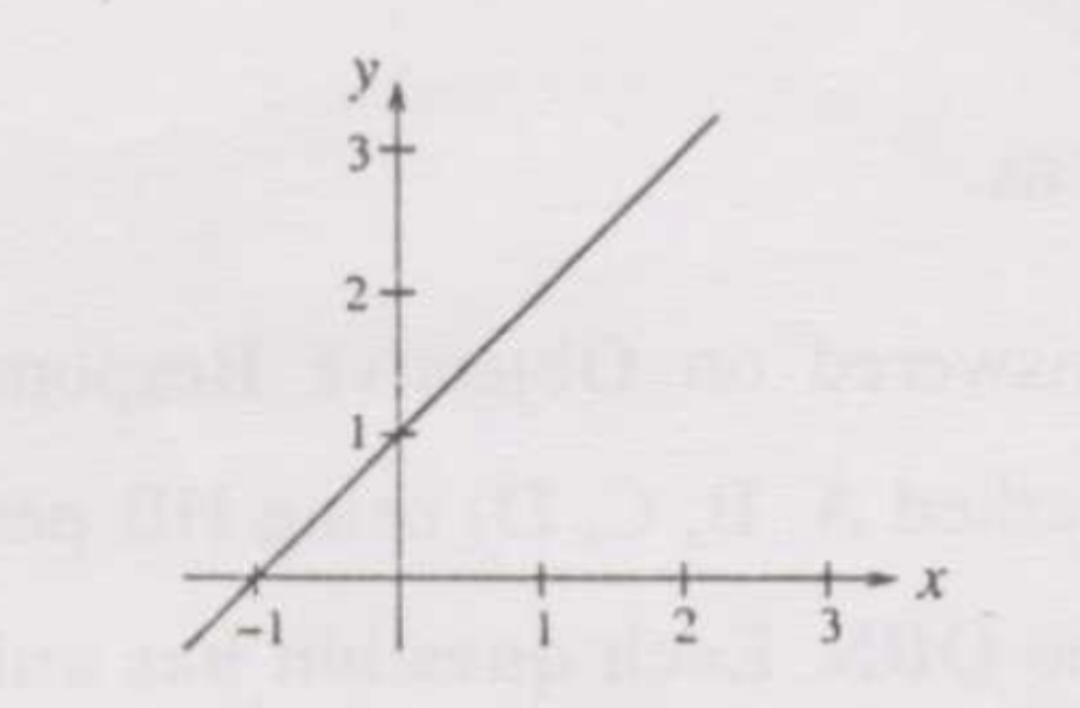
\includegraphics[width=0.4\textwidth]{Q2.jpg}
    \caption{}
    \label{fig:Q2.jpg}
\end{figure}


\begin{enumerate}
\begin{multicols}{4}
    \item 1.0
    \item 2.5
    \item 4.0
    \item 5.0
\end{multicols} 
\end{enumerate}


\item For $|x| < 1 $, $ \coth(x)$ can be approximated as: 
\hfill{\brak{\text{GATE EE 2025}}}
\begin{enumerate}
\begin{multicols}{4}
    \item $ x $
    \item $ x^2 $
    \item $ \frac{1}{x} $
    \item $ \frac{1}{x^2} $
\end{multicols} 
\end{enumerate}

\item $ \lim_{\theta \to 0} \frac{\sin(\theta/2)}{\theta} $ is: 
\hfill{\brak{\text{GATE EE 2025}}}
\begin{enumerate}
\begin{multicols}{4}
    \item 0.5
    \item 1
    \item 2
    \item Not defined
\end{multicols} 
\end{enumerate}

\item Which of the following functions is strictly bounded? 
\hfill{\brak{\text{GATE EE 2025}}}
\begin{multicols}{4}
\begin{enumerate}
    \item $ \sin x $
    \item $ e^x $
    \item $ cos x $
    \item $ x^2 $
\end{enumerate}
\end{multicols}

\item For the function $ e^{-x} $, the linear approximation around $ x = 2 $ is:
\hfill{\brak{\text{GATE EE 2025}}}
\begin{enumerate}
    \item $ (3 - x)^2 $
    \item $ 1 - x $
    \item $ [3 + 2\sqrt{2} - (1 + \sqrt{2})x]e^2 $
    \item $ e^{-2} $
\end{enumerate}

\item An independent voltage source in series with $ Z_s = R_s + jX_s $ delivers max average power to load $ Z_L $ when:
\hfill{\brak{\text{GATE EE 2025}}}
\begin{enumerate}
    \item $ Z_L = R_s + jX_s $
    \item $ Z_L = R_s $
    \item $ Z_L = jX_s $
    \item $ Z_L = R_s - jX_s $
\end{enumerate}


\item The RC circuit shown is:

\begin{figure}[ht!]
    \centering
    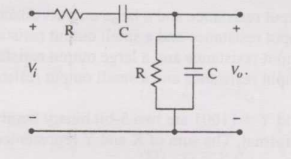
\includegraphics[width=0.4\textwidth]{Q8.png}
    \caption{}
    \label{fig:Q8.png}
\end{figure}

\hfill{\brak{\text{GATE EE 2025}}}
\begin{multicols}{4}
\begin{enumerate}
    \item Low-pass filter
    \item High-pass filter
    \item Band-pass filter
    \item Band-reject filter
\end{enumerate}
\end{multicols}

\item The electron and hole concentrations in an intrinsic semiconductor are $ n_i $ per cm$^3$ at 300 K. If acceptor impurities are introduced with concentration $ N_a $, then electron concentration becomes:
\hfill{\brak{\text{GATE EE 2025}}}
\begin{multicols}{4}
\begin{enumerate}
    \item $ n_i $
    \item $ n_i + N_a $
    \item $ N_a - n_i $
    \item $ \frac{n_i^2}{N_a} $
\end{enumerate}
\end{multicols}

\item In a $ p^+n $ junction diode under reverse bias, electric field is maximum at:
\hfill{\brak{\text{GATE EE 2025}}}

\begin{enumerate}
    \item Edge of depletion region on p-side
    \item Edge on n-side
    \item The junction
    \item Centre of depletion on n-side
\end{enumerate}

\item The correct full wave rectifier circuit is:
\begin{figure}[ht!]
    \centering
    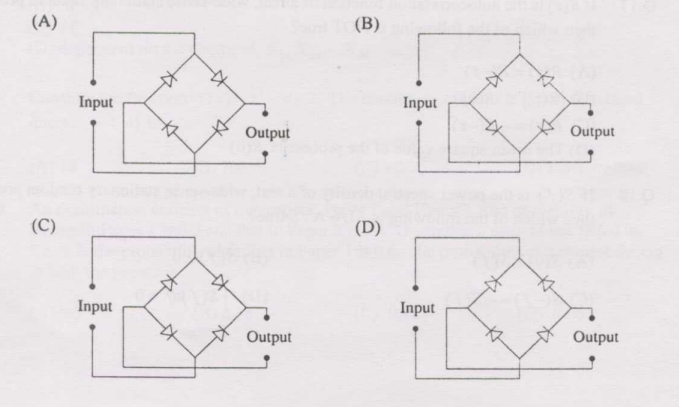
\includegraphics[width=0.75\textwidth]{Q11.png}
    \caption{}
    \label{fig:Q11.png}
\end{figure}

\hfill{\brak{\text{GATE EE 2025}}}
\item In a transconductance amplifier, it is desirable to have: 
\hfill{\brak{\text{GATE EE 2025}}}
\begin{enumerate}
    \item Large input and output resistance
    \item Large input and small output resistance
    \item Small input and large output resistance
    \item Small input and output resistance
\end{enumerate}

\item $ X = 01110 $, $ Y = 11001 $ (5-bit numbers in 2's complement). The sum in 6 bits is: 
\hfill{\brak{\text{GATE EE 2025}}}
\begin{multicols}{4}

\begin{enumerate}
    \item 100111
    \item 001100
    \item 000111
    \item 101001
\end{enumerate}
\end{multicols}

\item The Boolean function $ Y = AB + CD $ using only 2-input NAND gates requires: 
\hfill{\brak{\text{GATE EE 2025}}}
\begin{multicols}{4}
\begin{enumerate}
    \item 2
    \item 3
    \item 4
    \item 5
\end{enumerate}
\end{multicols}


\item Given closed-loop transfer function $ T(s) = \frac{s - 5}{(s+2)(s+3)} $, the system is: 
\hfill{\brak{\text{GATE EE 2025}}}
\begin{enumerate}
    \item Unstable
    \item Uncontrollable
    \item Minimum phase
    \item Non-minimum phase
\end{enumerate}

\item If Laplace transform of $ y(t) $ is $ Y(s) = \frac{1}{s(s - 1)} $, the final value is:
\hfill{\brak{\text{GATE EE 2025}}}
\begin{multicols}{4}
\begin{enumerate}
    \item $-1$
    \item $0$
    \item $1$
    \item Unbounded
\end{enumerate}
\end{multicols}

\item If $ R(\tau) $ is autocorrelation of real, WSS random process, which is NOT true: 
\hfill{\brak{\text{GATE EE 2025}}}
\begin{enumerate}
    \item $ R(\tau) = R(-\tau) $
    \item $ |R(t)| \leq R(0) $
    \item $ R(\tau) = -R(-\tau) $
    \item Mean square value is $ R(0) $
\end{enumerate}

\item If $ S(f) $ is power spectral density of a real WSS random process, which is ALWAYS true: 

\hfill{\brak{\text{GATE EE 2025}}}
\begin{multicols}{4}
\begin{enumerate}
    \item $ S(0) \geq S(f) $
    \item $ S(f) \geq 0 $
    \item $ S(-f) = -S(f) $
    \item $ \int S(f) df = 0 $
\end{enumerate}
\end{multicols}

\item A plane wave of wavelength $\lambda$ is travelling in a direction making an angle $30^\circ$ with positive x-axis and $90^\circ$ with positive y-axis. The $\mathbf{E}$ field of the plane wave can be represented as $(E_0 \text{ is a constant})$ 
\hfill{\brak{\text{GATE EE 2025}}}

\begin{flalign*}
    &\text{(A) }\mathbf{E} = -\hat{z},\ E_0\, \exp\left(j\left(\omega t - \frac{\sqrt{3}}{2}k x - \frac{1}{2}k y\right)\right) && \\
    &\text{(B) }\mathbf{E} = -\hat{z},\ E_0\, \exp\left(j\left(\omega t - \frac{\sqrt{3}}{2}k y\right)\right) && \\
    &\text{(C) }\mathbf{E} = -\hat{z},\ E_0\, \exp\left(j\left(\omega t + \frac{\sqrt{3}}{2}k x + \frac{1}{2}k y\right)\right) && \\
    &\text{(D) }\mathbf{E} = -\hat{z},\ E_0\, \exp\left(j\left(\omega t - \frac{\sqrt{3}}{2}k x + \frac{1}{2}k y\right)\right) &&
\end{flalign*}


\item If $C$ is a closed curve enclosing a surface $S$, then the magnetic field intensity $\mathbf{H}$, the current density $\mathbf{J}$ and the electric flux density $\mathbf{D}$ are related by 
\hfill{\brak{\text{GATE EE 2025}}}

    \begin{flalign*}
    &\text{(A) } \displaystyle \int_S \mathbf{H} \cdot d\mathbf{s} = \int_S \left(\mathbf{J} + \frac{\partial \mathbf{D}}{\partial t}\right) \cdot d\mathbf{s} && \\
    &\text{(B) } \displaystyle \oint_C \mathbf{H} \cdot d\mathbf{l} = \int_S \left(\mathbf{J} + \frac{\partial \mathbf{D}}{\partial t}\right) \cdot d\mathbf{s} && \\
    &\text{(C) } \displaystyle \int_S \mathbf{H} \cdot d\mathbf{s} = \oint_C \left(\mathbf{J} + \frac{\partial \mathbf{D}}{\partial t}\right) \cdot d\mathbf{l} && \\
    &\text{(D) } \displaystyle \oint_C \mathbf{H} \cdot d\mathbf{l} = \oint_C \left(\mathbf{J} + \frac{\partial \mathbf{D}}{\partial t}\right) \cdot d\mathbf{l} &&
\end{flalign*}


\item It is given that $X_1, X_2, \ldots, X_M$ are $M$ non-zero, orthogonal vectors. The dimension of the vector space spanned by the $2M$ vectors $X_1, X_2, \ldots, X_M, -X_1\\, -X_2, \ldots, -X_M$ is: 
\hfill{\brak{\text{GATE EE 2025}}}

\begin{enumerate}[label=(\Alph*)]
    \item $2M$
    \item $M+1$
    \item $M$
    \item \text{Dependent on choice of } $X_i$
\end{enumerate}

\item Consider the function $f(x) = x^2 - x -2$. The maximum value of $f(x)$ in the closed interval $[-4,4]$ is:
\hfill{\brak{\text{GATE EE 2025}}}
\begin{multicols}{4}
\begin{enumerate}
    \item 18
    \item 10
    \item $-2.25$
    \item Indeterminate
\end{enumerate}
\end{multicols}

\item An examination consists of two papers, Paper I and Paper II. The probability of failing in Paper I is 0.3 and that in Paper II is 0.2. Given that a student has failed in Paper II, the probability of failing in Paper I is 0.6. The probability of a student failing in both the papers is: 
\hfill{\brak{\text{GATE EE 2025}}}
\begin{multicols}{4}
\begin{enumerate}
    \item 0.5
    \item 0.18
    \item 0.12
    \item 0.06
\end{enumerate}
\end{multicols}{}

\item The solution of the differential equation $k^2 \frac{d^2 y}{dx^2} = y$, under the boundary conditions (i) $y = y_1$ at $x = 0$ and (ii) $y = y_2$ at $x = \infty$, where $k, y_1, y_2$ are constants, is: 
\hfill{\brak{\text{GATE EE 2025}}}
\begin{flalign*}
     &\text{(A) } y = (y_1 - y_2)\exp(-x/k) + y_2 && \\
    &\text{(B) } y = (y_1 - y_2)\exp(-x/k) + y_1 && \\
    &\text{(C) } y = (y_1 - y_2)\sinh(x/k) + y_2 && \\
    &\text{(D) } y = (y_1 - y_2)\exp(-x/k) + y_1 &&
\end{flalign*}
    
\item The equation $x^2 + x^4 - 4x - 4 = 0$ is to be solved using Newton-Raphson. If $x = 2$ is the initial approximation, then the next approximation using this method will be:
\hfill{\brak{\text{GATE EE 2025}}}

\begin{multicols}{4}
\begin{enumerate}
    \item $\frac{2}{3}$
    \item $\frac{4}{3}$
    \item $1$
    \item $\frac{3}{2}$   
\end{enumerate}
\end{multicols}

\item Three functions $f_1(t), f_2(t)$ and $f_3(t)$, which are zero outside the interval $[0,7]$, are shown in the figure. Which of the following statements is correct? 

\begin{figure}[ht!]
    \centering
    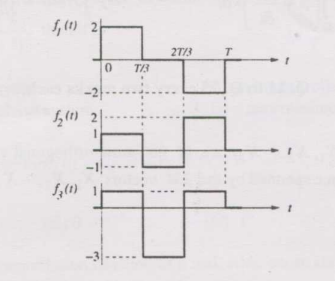
\includegraphics[width=0.6\textwidth]{Q26.png}
    \caption{}
    \label{fig:Q26.png}
\end{figure}


\hfill{\brak{\text{GATE EE 2025}}}
\begin{enumerate}[label=(\Alph*)]
    \item $f_1(t)$ and $f_2(t)$ are orthogonal
    \item $f_1(t)$ and $f_3(t)$ are orthogonal
    \item $f_2(t)$ and $f_3(t)$ are orthogonal
    \item $f_1(t)$ and $f_2(t)$ are orthonormal
\end{enumerate}

\item If the semi-circular contour $D$ of radius 2 is as shown in the figure, then the value of the integral $\displaystyle \oint_D \frac{1}{(s^2 -1)} ds$ is: 

\begin{figure}[ht!]
    \centering
    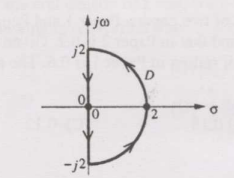
\includegraphics[width=0.4\textwidth]{Q27.png}
    \caption{}
    \label{fig:Q27.png}
\end{figure}

\hfill{\brak{\text{GATE EE 2025}}}
\begin{multicols}{4}
\begin{enumerate}[label=(\Alph*)]
    \item $j\pi$
    \item $-j\pi$
    \item $-\pi$
    \item $\pi$
\end{enumerate}
\end{multicols}

\item Two series resonant filters are as shown in the figure. Let the 3-dB bandwidth of Filter 1 be $B_1$ and that of Filter 2 be $B_2$. The value of $\frac{B_1}{B_2}$ is: 

\hfill{\brak{\text{GATE EE 2025}}}
\begin{figure}[ht!]
    \centering
    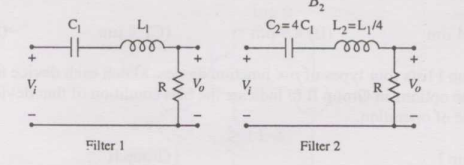
\includegraphics[width=0.6\textwidth]{Q28.png}
    \caption{}
    \label{fig:Q28.png}
\end{figure}


\begin{multicols}{4}
\begin{enumerate}[label=(\Alph*)]
    \item 4
    \item 1
    \item $\dfrac{1}{2}$
    \item $\dfrac{1}{4}$
\end{enumerate}
\end{multicols}

\item For the circuit shown in the figure, the Thevenin voltage and resistance looking into XY are: 
\hfill{\brak{\text{GATE EE 2025}}}
\begin{multicols}{4}
\begin{enumerate}
    \item $\frac{4}{3}$ V, $2\,\Omega$
    \item $4$ V, $\frac{2}{3}\,\Omega$
    \item $\frac{4}{3}$ V, $\frac{2}{3}\,\Omega$
    \item $4$ V, $2\,\Omega$
\end{enumerate}
\end{multicols}

\item In the circuit shown, $V_C$ is 0 volts at $t=0$ sec. For $t>0$, the capacitor current $i_c(t)$, where $t$ is in seconds, is given by: 
\hfill{\brak{\text{GATE EE 2025}}}

\begin{figure}[ht!]
    \centering
    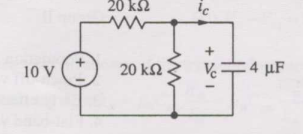
\includegraphics[width=0.5\textwidth]{Q30.png}
    \caption{}
    \label{fig:Q30.png}
\end{figure}

\begin{enumerate}
  \item $0.50\exp(-25t)\,$mA
  \item $0.25\exp(-25t)\,$mA
  \item $0.50\exp(-12.5t)\,$mA
  \item $0.25\exp(-6.25t)\,$mA
\end{enumerate}

\item In the AC network shown in the figure, the phasor voltage $V_{AB}$ (in Volts) is: 

\begin{figure}[ht!]
    \centering
    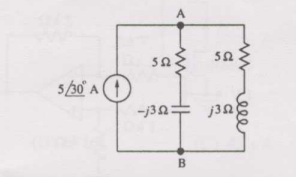
\includegraphics[width=0.4\textwidth]{Q31.png}
    \caption{}
    \label{fig:Q31.png}
\end{figure}

\hfill{\brak{\text{GATE EE 2025}}}
\begin{multicols}{4}

\begin{enumerate}
    \item 0
    \item $5\angle 20^\circ$
    \item $12.5\angle 30^\circ$
    \item $17\angle 30^\circ$
\end{enumerate}
\end{multicols}

\item A p$^+$n junction has a built-in potential of 0.8 V. The depletion layer width at a reverse bias of 1.2 V is 2 $\mu$m. For a reverse bias of 7.2 V, the depletion layer width will be:
\hfill{\brak{\text{GATE EE 2025}}}
\begin{multicols}{4}
\begin{enumerate}
    \item 4 $\mu$m
    \item 4.9 $\mu$m
    \item 8 $\mu$m
    \item 12 $\mu$m
\end{enumerate}
\end{multicols}

\item Group I lists four types of pn junction diodes. Match each device in Group I with one of the options in Group II to indicate the bias condition of that device in its normal mode of operation. 

\resizebox{0.5\textwidth}{!}{%
\begin{tabular}{|c|l|c|l|}
\hline
Group I & Device              & Group II & Bias Condition   \\
\hline
P       & Zener Diode         & 1        & Forward bias     \\
Q       & Solar cell          & 2        & Reverse bias     \\
R       & LASER diode         &          &                 \\
S       & Avalanche Photodiode&          &                 \\
\hline
\end{tabular}
}

\hfill{\brak{\text{GATE EE 2025}}}
\begin{enumerate}
    \item P-1, Q-2, R-1, S-2
    \item P-2, Q-1, R-1, S-2
    \item P-2, Q-2, R-1, S-1
    \item P-2, Q-1, R-2, S-2
\end{enumerate}

\item The DC current gain ($\beta$) of a BJT is 50. Assuming that the emitter injection efficiency is 0.995, the base transport factor is:
\hfill{\brak{\text{GATE EE 2025}}}

\begin{multicols}{4}
\begin{enumerate}
  \item 0.980
  \item 0.985
  \item 0.990
  \item 0.995
\end{enumerate}
\end{multicols}

\item Group I lists four different semiconductor devices. Match each device in Group I with its characteristic property in Group II. 

\resizebox{0.5\textwidth}{!}{
  \begin{tabular}{|c|l|c|l|}
  \hline
  Group I & Device         & Group II & Property            \\
  \hline
  P       & BJT            & 1        & Population inversion \\
  Q       & MOS capacitor  & 2        & Pinch-off voltage   \\
  R       & LASER diode    & 3        & Early effect        \\
  S       & JFET           & 4        & Flat-band voltage   \\
  \hline
  \end{tabular}
}
\hfill{\brak{\text{GATE EE 2025}}}

\begin{enumerate}
    \item P-3, Q-1, R-4, S-2
    \item P-1, Q-4, R-3, S-2
    \item P-3, Q-4, R-1, S-2
    \item P-3, Q-2, R-1, S-4
\end{enumerate}

\item For the Op-Amp circuit shown in the figure, $V_o$ is: 

\begin{figure}[ht!]
    \centering
    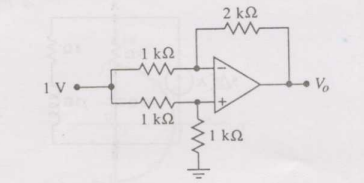
\includegraphics[width=0.4\textwidth]{Q36.png}
    \caption{}
    \label{fig:Q36.png}
\end{figure}

\hfill{\brak{\text{GATE EE 2025}}}

\begin{multicols}{4}
\begin{enumerate}
  \item $-2$ V
  \item $-1$ V
  \item $-0.5$ V
  \item $0.5$ V
\end{enumerate}
\end{multicols}

\item For the BJT circuit shown, assume that the $\beta$ of the transistor is very large and $V_{BE} = 0.7\text{ V}$. The mode of operation of the BJT is: 

\begin{figure}[ht!]
    \centering
    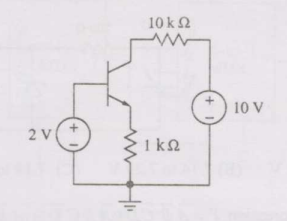
\includegraphics[width=0.5\textwidth]{Q37.png}
    \caption{}
    \label{fig:Q37.png}
\end{figure}

\hfill{\brak{\text{GATE EE 2025}}}
\begin{multicols}{4}
\begin{enumerate}
  \item cut-off
  \item saturation
  \item normal active
  \item reverse active
\end{enumerate}
\end{multicols}

\item In the op-amp circuit shown, assume that the diode current follows the equation $I = I_S \exp(V/V_T)$. For $V_i = 2\text{ V}$, $V_o = V_{o1}$, and for $V_i = 4\text{ V}$, $V_o = V_{o2}$. The relationship between $V_{o1}$ and $V_{o2}$ is: 

\begin{figure}[ht!]
    \centering
    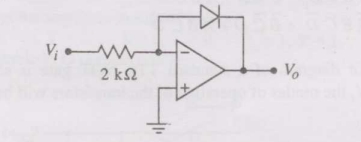
\includegraphics[width=0.4\textwidth]{Q38.png}
    \caption{}
    \label{fig:Q38.png}
\end{figure}


\hfill{\brak{\text{GATE EE 2025}}}
\begin{enumerate}
  \item $V_{o2} = \sqrt{2}\,V_{o1}$
  \item $V_{o2} = e^2 V_{o1}$
  \item $V_{o2} = V_{o1} \ln 2$
  \item $V_{o1} - V_{o2} = V_T \ln 2$
\end{enumerate}

\item In the CMOS inverter circuit shown, if the transconductance parameters of the NMOS and PMOS transistors are $k_n = k_p = \mu C_{ox}\frac{W_n}{L_n} = \mu C_{ox}\frac{W_p}{L_p} = 40~\mu\text{A}/\text{V}^2$ and their threshold voltages are $V_{THn} = |V_{THp}| = 1\text{ V}$, the current $I$ is: 

\begin{figure}[ht!]
    \centering
    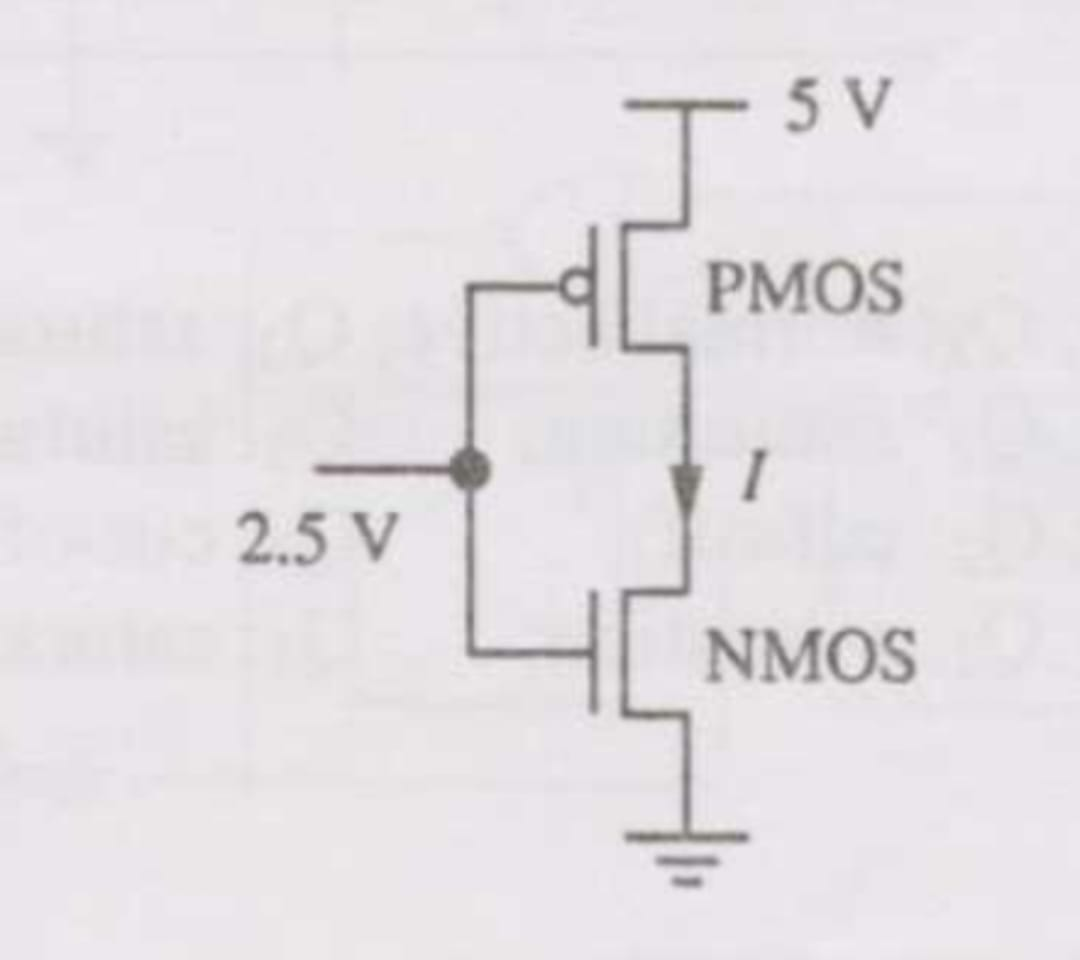
\includegraphics[width=0.4\textwidth]{Q39.jpg}
    \caption{}
    \label{fig:Q39.jpg}
\end{figure}

\hfill{\brak{\text{GATE EE 2025}}}

\begin{multicols}{4}
\begin{enumerate}[label=(\Alph*)]
  \item $0~\text{A}$
  \item $25~\mu\text{A}$
  \item $45~\mu\text{A}$
  \item $90~\mu\text{A}$
\end{enumerate}
\end{multicols}

\item For the Zener diode shown in the figure, the Zener voltage at knee is 7 V, the knee current is negligible and the Zener dynamic resistance is $10~\Omega$. If the input voltage ($V_i$) range is from 10 to 16 V, the output voltage ($V_o$) ranges from: 

\begin{figure}[ht!]
    \centering
    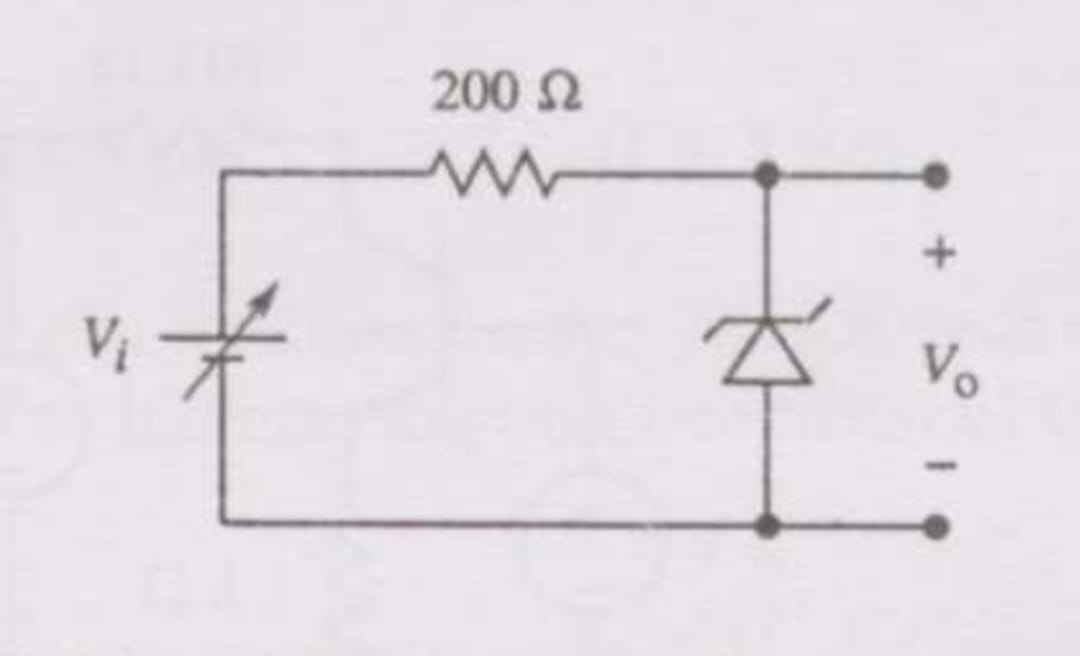
\includegraphics[width=0.4\textwidth]{Q40.jpg}
    \caption{}
    \label{fig:Q40.jpg}
\end{figure}

\hfill{\brak{\text{GATE EE 2025}}}
\begin{enumerate}[label=(\Alph*)]
    \item $7.00$ to $7.29$ V
    \item $7.14$ to $7.29$ V
    \item $7.14$ to $7.43$ V
    \item $7.29$ to $7.43$ V
\end{enumerate}

\item The Boolean expression  
$
Y = \overline{A} \,\overline{B}\,\overline{C} D + \overline{A} B C \overline{D} + A \overline{B} C \overline{D} + A B \overline{C} \overline{D}
$
can be minimized to: 
\hfill{\brak{\text{GATE EE 2025}}}
\begin{enumerate}
  \item $\overline{A} \,\overline{B} C \overline{D} + \overline{A} B \overline{C} + A \overline{C} \overline{D}$
  \item $\overline{A} \,\overline{B} C \overline{D} + B \overline{C} \overline{D} + A \overline{B} \overline{C} D$
  \item $\overline{A} B C \overline{D} + \overline{B} C \overline{D} + A B \overline{C} D$
  \item $\overline{A} B \overline{C} D + \overline{B} \overline{C} D + A B \overline{C} \overline{D}$
\end{enumerate}

\item The circuit diagram of a standard TTL NOT gate is shown. When $V_i = 2.5\text{ V}$, the modes of operation of the transistors will be: 

\begin{figure}[H]
    \centering
    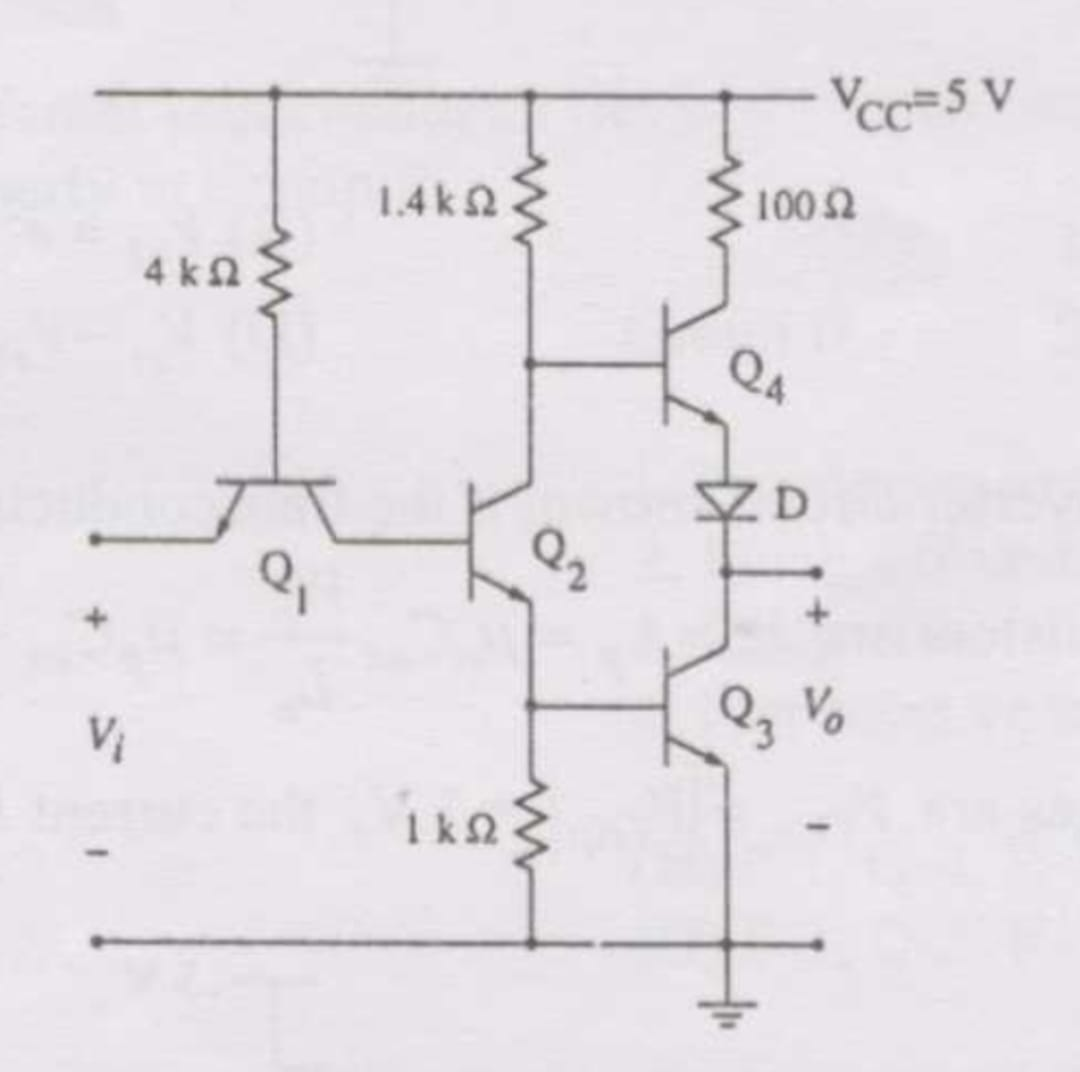
\includegraphics[width=0.4\linewidth]{Q42.jpg}
    \caption{circuit}
    \label{fig:full_wave}
\end{figure}

\hfill{\brak{\text{GATE EE 2025}}}
\begin{enumerate}
  \item $Q_1$: reverse active; $Q_2$: normal active; $Q_3$: saturation; $Q_4$: cut-off
  \item $Q_1$: reverse active; $Q_2$: saturation; $Q_3$: saturation; $Q_4$: cut-off
  \item $Q_1$: normal active; $Q_2$: cut-off; $Q_3$: cut-off; $Q_4$: saturation
  \item $Q_1$: saturation; $Q_2$: saturation; $Q_3$: saturation; $Q_4$: normal active
\end{enumerate}

\item In the following circuit, $X$ is given by: 

\begin{figure}[ht!]
    \centering
    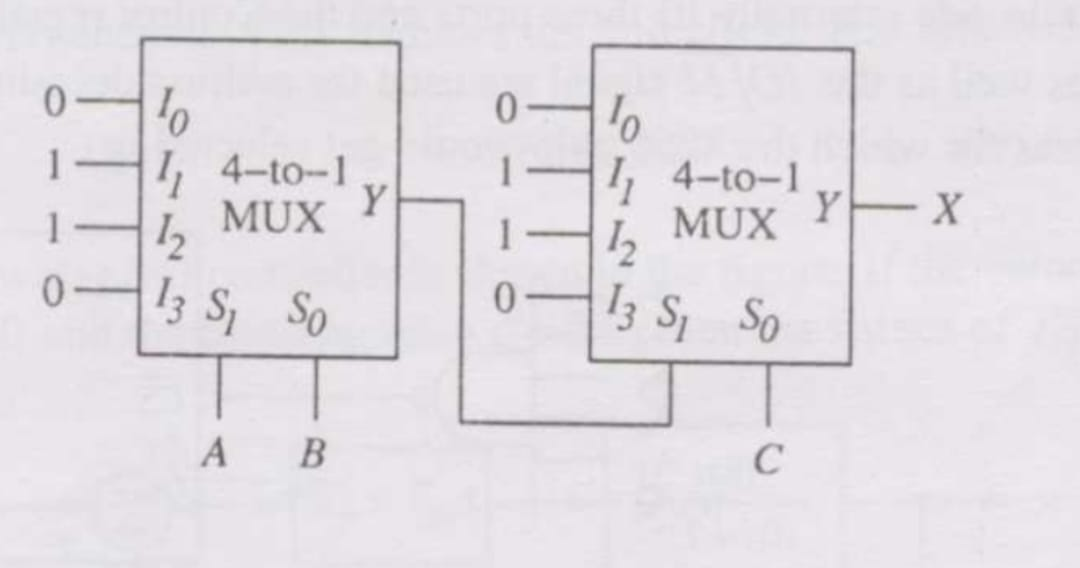
\includegraphics[width=0.6\textwidth]{Q43.jpg}
    \caption{}
    \label{fig:Q43.jpg}
\end{figure}

\hfill{\brak{\text{GATE EE 2025}}}
\begin{enumerate}
  \item $X = \overline{A} \,\overline{B} C + \overline{A} B \overline{C} + \overline{A} B C + A B C$
  \item $X = \overline{A} B C + \overline{A} B \overline{C} + A B \overline{C} + \overline{A} \overline{B} C$
  \item $X = A B + B C + A C$
  \item $X = \overline{A} B + \overline{B} \overline{C} + A \overline{C}$
\end{enumerate}

\item The following binary values were applied to the X and Y inputs of the NAND latch shown. The corresponding stable P, Q outputs will be: 

\begin{figure}[ht!]
    \centering
    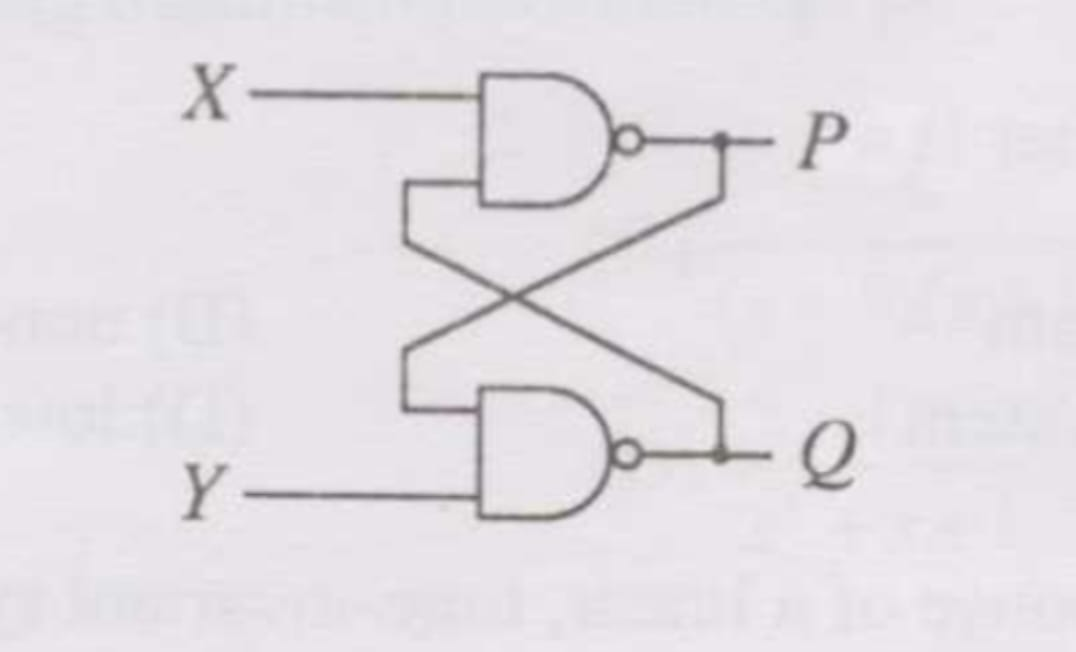
\includegraphics[width=0.4\textwidth]{Q44.jpg}
    \caption{}
    \label{fig:Q44.jpg}
\end{figure}

 Applied sequence: $X=0,Y=1$; then $X=0,Y=0$; then $X=1,Y=1$.
\hfill{\brak{\text{GATE EE 2025}}}
\begin{enumerate}
  \item $P=1,\ Q=0$; \quad $P=1,\ Q=0$; \quad $P=1,\ Q=0$
  \item $P=1,\ Q=0$; \quad $P=0,\ Q=1$ or $P=0,\ Q=1$; \quad $P=0,\ Q=1$
  \item $P=1,\ Q=0$; \quad $P=1,\ Q=1$; \quad $P=1,\ Q=0$ or $P=0,\ Q=1$
  \item $P=1,\ Q=0$; \quad $P=1,\ Q=1$; \quad $P=1,\ Q=1$
\end{enumerate}

\item For the circuit shown, the counter state $(Q_1 Q_0)$ follows the sequence:

\begin{figure}[H]
    \centering
    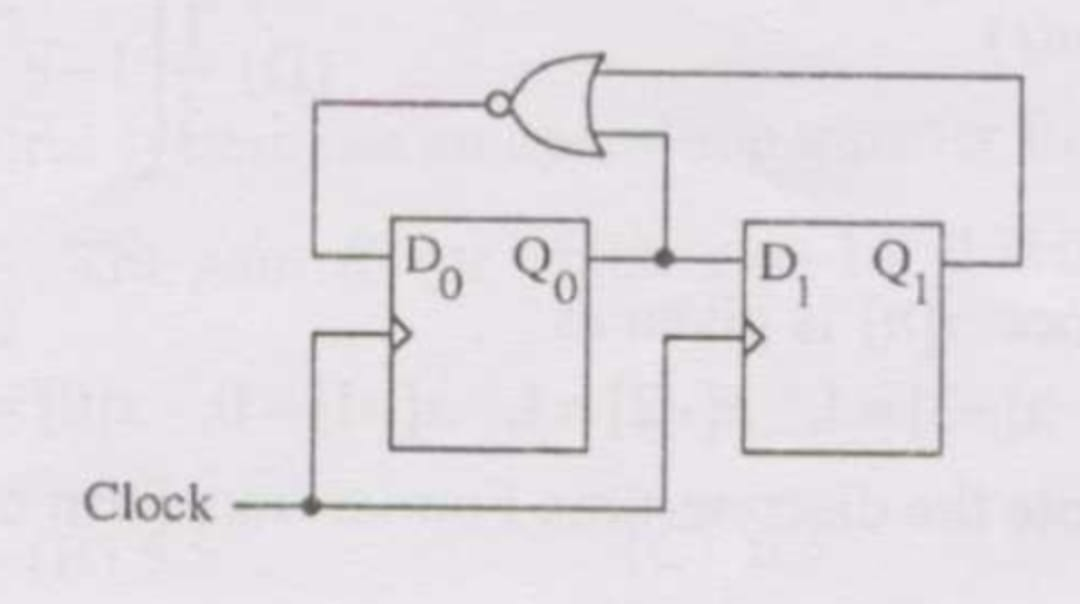
\includegraphics[width=0.4\linewidth]{Q45.jpg}
    \caption{circuit}
    \label{fig:full_wave}
\end{figure}

\hfill{\brak{\text{GATE EE 2025}}}
\begin{enumerate}
  \item $00,\ 01,\ 10,\ 11,\ 00,\dots$
  \item $00,\ 01,\ 10,\ 00,\ 01,\dots$
  \item $00,\ 01,\ 11,\ 00,\ 01,\dots$
  \item $00,\ 10,\ 11,\ 00,\ 10,\dots$
\end{enumerate}

\item An 8255 chip is interfaced to an 8085 microprocessor system as an I/O mapped I/Os as shown. The address lines $A_0$ and $A_1$ of the 8085 are used by the 8255 chip to decode internally its three ports and the Control register. The address lines $A_3$ to $A_7$ as well as the IO/M signal are used for address decoding. The range of addresses for which the 8255 chip would get selected is: 

\begin{figure}[ht!]
    \centering
    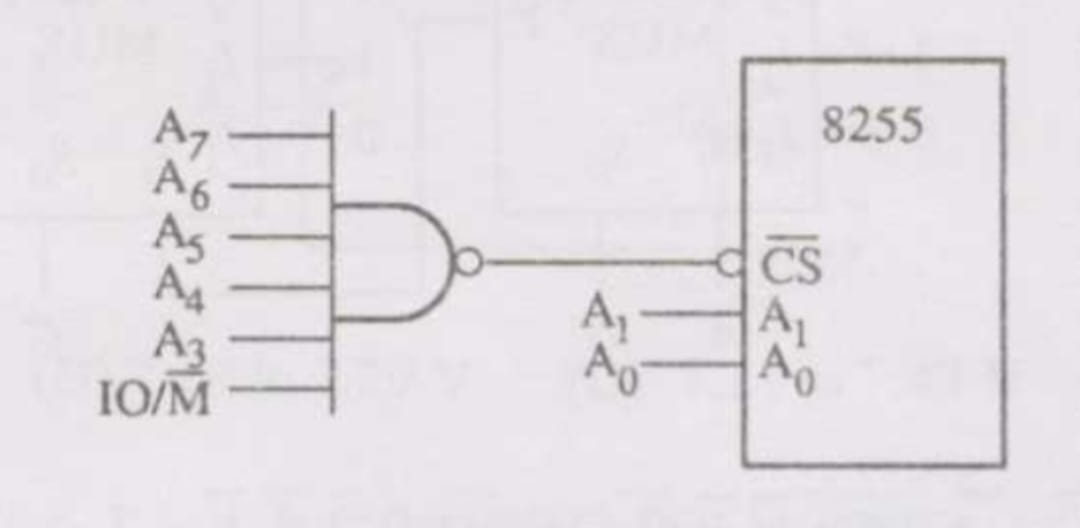
\includegraphics[width=0.4\textwidth]{Q46.jpg}
    \caption{}
    \label{fig:Q46.jpg}
\end{figure}

\hfill{\brak{\text{GATE EE 2025}}}
\begin{enumerate}
  \item F8H -- FBH
  \item F8H -- FCH
  \item F8H -- FFH
  \item F0H -- F7H
\end{enumerate}

\item The 3-dB bandwidth of the low-pass signal $e^{-t}u(t)$ is: 
\hfill{\brak{\text{GATE EE 2025}}}
\begin{multicols}{4}
\begin{enumerate}
  \item $\frac{1}{2\pi}$ Hz
  \item $\frac{1}{2\pi}\sqrt{2}-1$ Hz
  \item $\infty$
  \item $1$ Hz
\end{enumerate}
\end{multicols}

\item A Hilbert transformer is a: 
\hfill{\brak{\text{GATE EE 2025}}}
\begin{enumerate}

  \item Non-linear system
  \item Non-causal system
  \item Time-varying system
  \item Low-pass system
\end{enumerate}

\item The frequency response of a linear time-invariant system is given by
$
H(f)=\frac{5}{1+j10\pi f}.
$

The step response of the system is: 
\hfill{\brak{\text{GATE EE 2025}}}
\begin{multicols}{2}
\begin{enumerate}
  \item $5\left(1-e^{-5t}\right)u(t)$
  \item $5\left(1-e^{-t/5}\right)u(t)$
  \item $\dfrac{1}{5}\left(1-e^{-5t}\right)u(t)$
  \item $\dfrac{1}{5}\left(1-e^{-t/5}\right)u(t)$
\end{enumerate}
\end{multicols}

\item
A 5-point sequence $x[n]$ is given as $x[-3]=1$, $x[-2]=1$, $x[-1]=0$,\\
$x[0]=5$, $x[1]=15$. Let $X\left(e^{j\omega}\right)$ denote the discrete-time Fourier\\
transform of $x[n]$. The value of
$
\int_{-\pi}^{\pi} X\left(e^{4j\omega3}\right)\, d\omega
$
\hfill{\brak{\text{GATE EE 2025}}}
\begin{multicols}{4}
\begin{enumerate}
  \item 5
  \item $10\pi$
  \item $16\pi$
  \item $5 + j10\pi$
\end{enumerate}
\end{multicols}

\item The $z$-transform $X[z]$ of a sequence $x[n]$ is given by
$
X[z]=\frac{0.5}{1-2z^{-1}}.
$

It is given that the region of convergence of $X[z]$ includes the unit circle. The value of $x[0]$ is: 
\hfill{\brak{\text{GATE EE 2025}}}
\begin{multicols}{4}
\begin{enumerate}
    \item $-0.5$
    \item $0$
    \item $0.25$
    \item $0.5$
\end{enumerate}
\end{multicols}

\item A control system with a PD controller is shown. If the velocity error constant $K_v=1000$ and the damping ratio $\zeta=0.5$, then the values of $K_P$ and $K_D$ are: 

\begin{figure}[ht!]
    \centering
    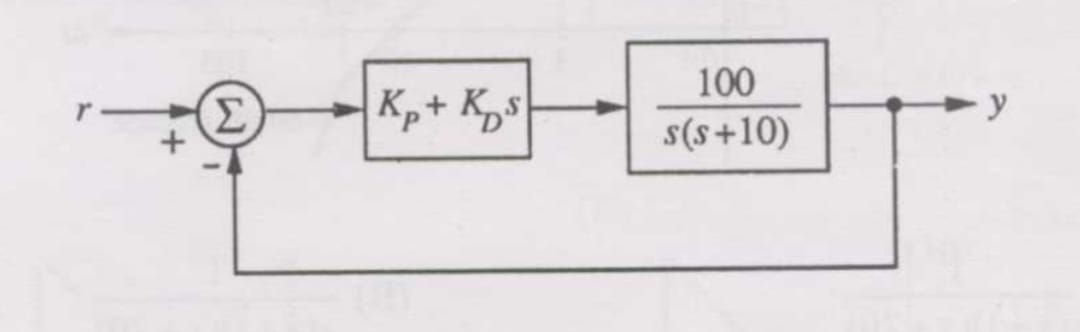
\includegraphics[width=0.4\textwidth]{Q52.jpg}
    \caption{}
    \label{fig:Q52.jpg}
\end{figure}

\hfill{\brak{\text{GATE EE 2025}}}
\begin{enumerate}
    \item $K_P=100,\ K_D=0.09$
    \item $K_P=100,\ K_D=0.9$
    \item $K_P=10,\ K_D=0.09$
    \item $K_P=10,\ K_D=0.9$
\end{enumerate}


\item The transfer function of a plant is
$
T(s)=\frac{5}{(s+5)(s^2+s+1)}.
$
The second-order approximation of $T(s)$ using the dominant pole concept is: 
\hfill{\brak{\text{GATE EE 2025}}}
\begin{multicols}{4}
\begin{enumerate}[label=(\Alph*)]
    \item $\frac{1}{(s+5)(s+1)}$
    \item $\frac{5}{(s+5)(s+1)}$
    \item $\frac{5}{s^2+s+1}$
    \item $\frac{1}{s^2+s+1}$
\end{enumerate}
\end{multicols}

\item The open-loop transfer function of a plant is given as $G(s)=\frac{1}{s^2-1}$. If the plant is operated in unity feedback, then the lead compensator that can stabilize the system is: 
\hfill{\brak{\text{GATE EE 2025}}}
\begin{multicols}{4}
\begin{enumerate}
    \item $\frac{10(s-1)}{s+2}$
    \item $\frac{10(s+4)}{s+2}$
    \item $\frac{10(s+2)}{s+10}$
    \item $\frac{2(s+2)}{s+10}$
\end{enumerate}
\end{multicols}

\item A unity feedback control system has an open-loop transfer function
$
G(s)=\frac{K}{s(s^2+7s+12)}.
$
The gain $K$ for which $s=-1+j1$ will lie on the root locus of this system is:
\hfill{\brak{\text{GATE EE 2025}}}
\begin{multicols}{4}
\begin{enumerate}
    \item 4
    \item 5.5
    \item 6.5
    \item 10
\end{enumerate}
\end{multicols}

\item The asymptotic Bode magnitude plot of a transfer function is as shown: starts at 60 dB, slopes $-20$ dB/decade until 1 rad/s (at 40 dB), then $-40$ dB/decade crossing 0 dB near 10, then $-60$ dB/decade. The transfer function $G(s)$ corresponding to this plot is: 
\hfill{\brak{\text{GATE EE 2025}}}
\begin{multicols}{4}
\begin{enumerate}
    \item $\frac{1}{(s+1)(s+20)}$
    \item $\frac{1}{s(s+1)(s+20)}$
    \item $\frac{100}{s(s+1)(s+20)}$
    \item $\frac{100}{s(s+1)(1+0.05s)}$
\end{enumerate}
\end{multicols}

 \item
    The state-space representation of a separately excited DC servo motor dynamics is given as
    $
    \frac{d}{dt}
    \myvec{
        \omega\quad\\
        i_a
    }
    =
    \myvec{
        -1\quad 1\\
        -1\quad -10
    }
    \myvec{
        \omega\quad\\
        i_a
    }
    +
    \myvec{
        0\\
        10
    }
    u
    $
    \quad where $\omega$ is the speed, $i_a$ is the armature current, and $u$ is the armature voltage. \quad

    The transfer function $\dfrac{\omega(s)}{u(s)}$ is: 
\hfill{\brak{\text{GATE EE 2025}}}
\begin{multicols}{4}
\begin{enumerate}
    \item $\dfrac{10}{s^2+11s+11}$
    \item $\dfrac{1}{s^2+11s+11}$
    \item $\dfrac{10s+10}{s^2+11s+11}$
    \item $\dfrac{1}{s^2+s+1}$
\end{enumerate}
\end{multicols}

\item In delta modulation, the slope overload distortion can be reduced by: 
\hfill{\brak{\text{GATE EE 2025}}}
\begin{enumerate}
    \item decreasing the step size
    \item decreasing the granular noise
    \item decreasing the sampling rate
    \item increasing the step size
\end{enumerate}

\item The raised cosine pulse $p(t)$ used for zero ISI with unity roll-off factor is
$
p(t)=\frac{\sin 4\pi W t}{4\pi W t(1-16W^2 t^2)}.
$
The value of $p(t)$ at $t=\dfrac{1}{4W}$ is:
\hfill{\brak{\text{GATE EE 2025}}}
\begin{multicols}{4}
\begin{enumerate}
    \item $-0.5$
    \item $0$
    \item $0.5$
    \item $\infty$
\end{enumerate}
\end{multicols}

\item In a GSM system, 8 channels coexist in 200 kHz using TDMA. A GSM operator is allocated 5 MHz. Assuming frequency reuse factor of $1/5$ (five-cell repeat), the maximum number of simultaneous channels in one cell is: 

\hfill{\brak{\text{GATE EE 2025}}}
\begin{multicols}{4}
\begin{enumerate}
  \item 200
  \item 40
  \item 25
  \item 5
\end{enumerate}
\end{multicols}

\item During transmission over a binary channel, bit errors occur independently with probability $p$. The probability of {at most one} bit in error in a block of $n$ bits is: 
\hfill{\brak{\text{GATE EE 2025}}}
\begin{multicols}{2}
    

\begin{enumerate}
    \item $p^n$
    \item $1-p^n$
    \item $np(1-p)^{n-1} + (1-p)^n$
    \item $1-(1-p)^n$
\end{enumerate}
\end{multicols}
\item In the following scheme, if the spectrum $M(f)$ of $m(t)$ is as shown, then the spectrum $Y(f)$ of $y(t)$ will be: 
\hfill{\brak{\text{GATE EE 2025}}}

\item In a Direct Sequence CDMA system the chip rate is $1.2288\times10^6$ chips/sec. If the processing gain is desired to be \textbf{at least} 100, the data rate:
\hfill{\brak{\text{GATE EE 2025}}}

\begin{enumerate}
  \item must be $\le 12.288\times10^3$ bits/sec
  \item must be $>12.288\times10^3$ bits/sec
  \item must be exactly $12.288\times10^3$ bits/sec
  \item can take any value less than $122.88\times10^3$ bits/sec
\end{enumerate}

\item An air-filled rectangular waveguide has inner dimensions $3\text{ cm}\times2\text{ cm}$. The wave impedance of the TE$_{20}$ mode at frequency 30 GHz is (free-space impedance $\eta_0=377~\Omega$): 
\hfill{\brak{\text{GATE EE 2025}}}

\begin{multicols}{4}
\begin{enumerate}
  \item $308~\Omega$
  \item $355~\Omega$
  \item $400~\Omega$
  \item $461~\Omega$
\end{enumerate}
\end{multicols}

\item The magnetic field of a plane wave in free space is
$
\mathbf{H} = \hat{x} \frac{5\sqrt{3}}{\eta_0} \cos(\omega t - \beta z)
+ \hat{y} \frac{5}{\eta_0} \left(-\sin(\omega t - \beta z + \frac{\pi}{2})\right).
$
The time-average power flow density in Watts is: 
\hfill{\brak{\text{GATE EE 2025}}}

\begin{multicols}{4}
\begin{enumerate}
  \item $\dfrac{\eta_0}{100}$
  \item $\dfrac{100}{\eta_0}$
  \item $50\eta_0^2$
  \item $\dfrac{50}{\eta_0}$
\end{enumerate}
\end{multicols}

\item The electric field in a rectangular waveguide of inner dimensions $a\times b$ is given by
$
\mathbf{E} = \frac{\omega\mu}{k^2} \left(\frac{\pi}{a}\right) H_0 \sin\left(\frac{2\pi x}{a}\right) \sin(\omega t - \beta z)\,\hat{y}.
$
The mode of propagation is: 
\hfill{\brak{\text{GATE EE 2025}}}
\begin{multicols}{4}
\begin{enumerate}
  \item TE$_{20}$
  \item TM$_{11}$
  \item TM$_{20}$
  \item TE$_{10}$
\end{enumerate}
\end{multicols}

\item The parallel branches of a 2-wire transmission line are terminated in $100~\Omega$ and $200~\Omega$ resistors as shown. The characteristic impedance of the line is $Z_0=50~\Omega$ and each section has length $\lambda/4$. The voltage reflection coefficient $\Gamma$ at the input is: 

\begin{figure}[ht!]
    \centering
    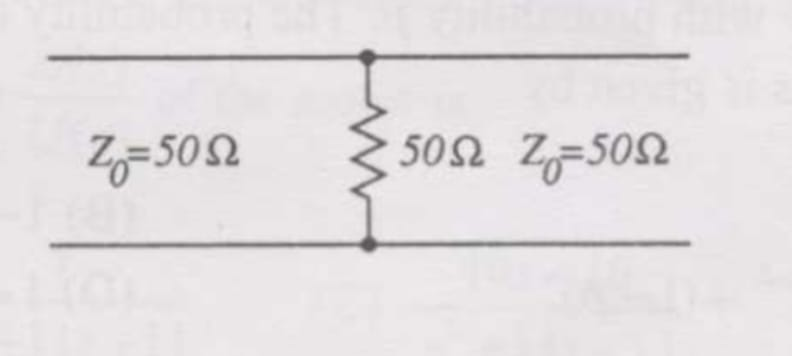
\includegraphics[width=0.4\textwidth]{Q67.jpg}
    \caption{}
    \label{fig:Q52.jpg}
\end{figure}
\hfill{\brak{\text{GATE EE 2025}}}

\begin{multicols}{4}
\begin{enumerate}
  \item $-j\frac{7}{5}$
  \item $-\frac{5}{7}$
  \item $j\frac{5}{7}$
  \item $\frac{5}{7}$
\end{enumerate}
\end{multicols}

\item A load of $50~\Omega$ is connected in shunt in a 2-wire transmission line of characteristic impedance $Z_0=50~\Omega$ as shown. The 2-port scattering parameter matrix (S-matrix) of the shunt element is: 

\begin{figure}[ht!]
    \centering
    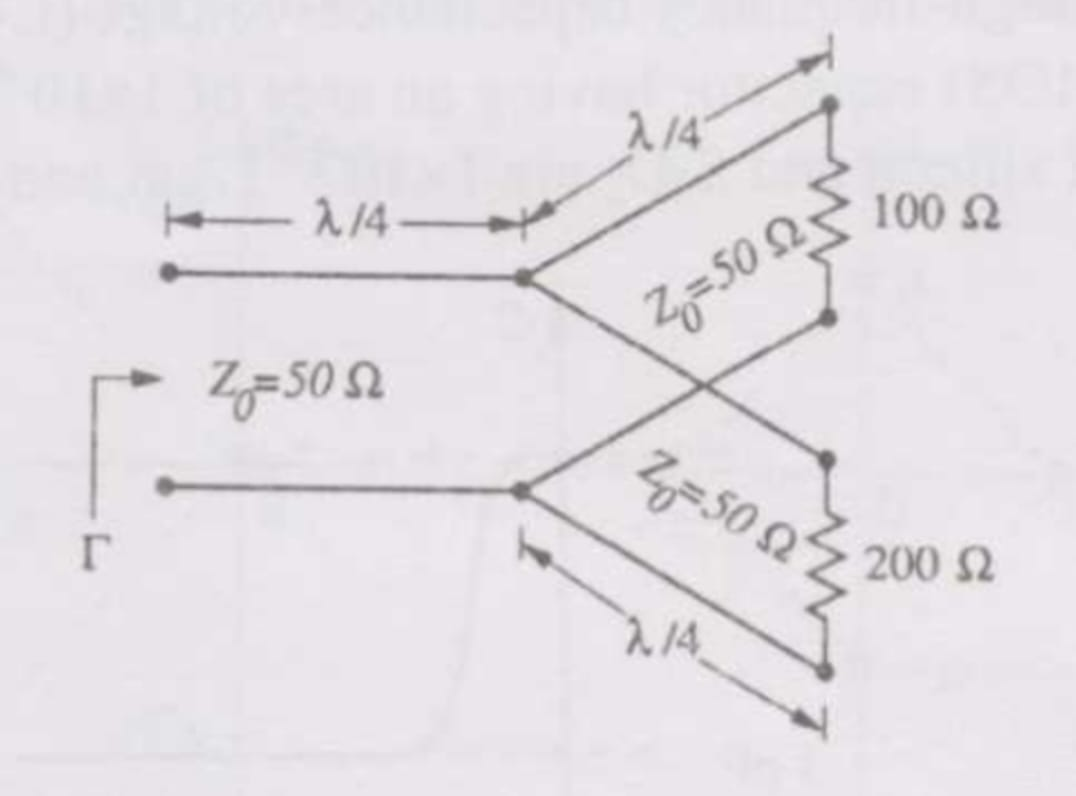
\includegraphics[width=0.3\textwidth]{Q68.jpg}
    \caption{}
    \label{fig:Q67.jpg}
\end{figure}
\hfill{\brak{\text{GATE EE 2025}}}

\begin{multicols}{4}
\begin{enumerate}
    \item $\myvec{\tfrac{1}{2} & \tfrac{1}{2} \\ \tfrac{1}{2} & \tfrac{1}{2}}$
    \item $\myvec{0 & 1 \\ 1 & 0}$
    \item $\myvec{\tfrac{1}{3} & \tfrac{2}{3} \\ \tfrac{2}{3} & \tfrac{1}{3}}$
    \item $\myvec{\tfrac{1}{4} & \tfrac{3}{4} \\ \tfrac{3}{4} & \tfrac{1}{4}}$
\end{enumerate}
\end{multicols}

\item A $\lambda/2$ dipole is kept horizontally at a height of $\lambda_0/2$ above a perfectly conducting ground plane. The radiation pattern in the plane of the dipole ($\vec{E}$-plane) looks approximately as: 

\begin{figure}[ht!]
    \centering
    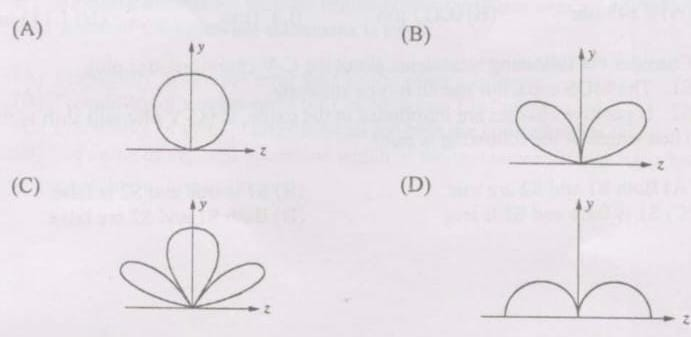
\includegraphics[width=0.6\textwidth]{Q69.jpg}
    \caption{}
    \label{fig:Q69.jpg}
\end{figure}
\hfill{\brak{\text{GATE EE 2025}}}

\begin{multicols}{4}
\begin{enumerate}
  \item A
  \item B
  \item C
  \item D
\end{enumerate}
\end{multicols}

\item A right circularly polarized (RCP) plane wave is incident at a dielectric interface. If the reflection coefficient $r_{l}=1$, the relative dielectric constant $\varepsilon_{r2}$ is:
\begin{figure}[ht!]
    \centering
    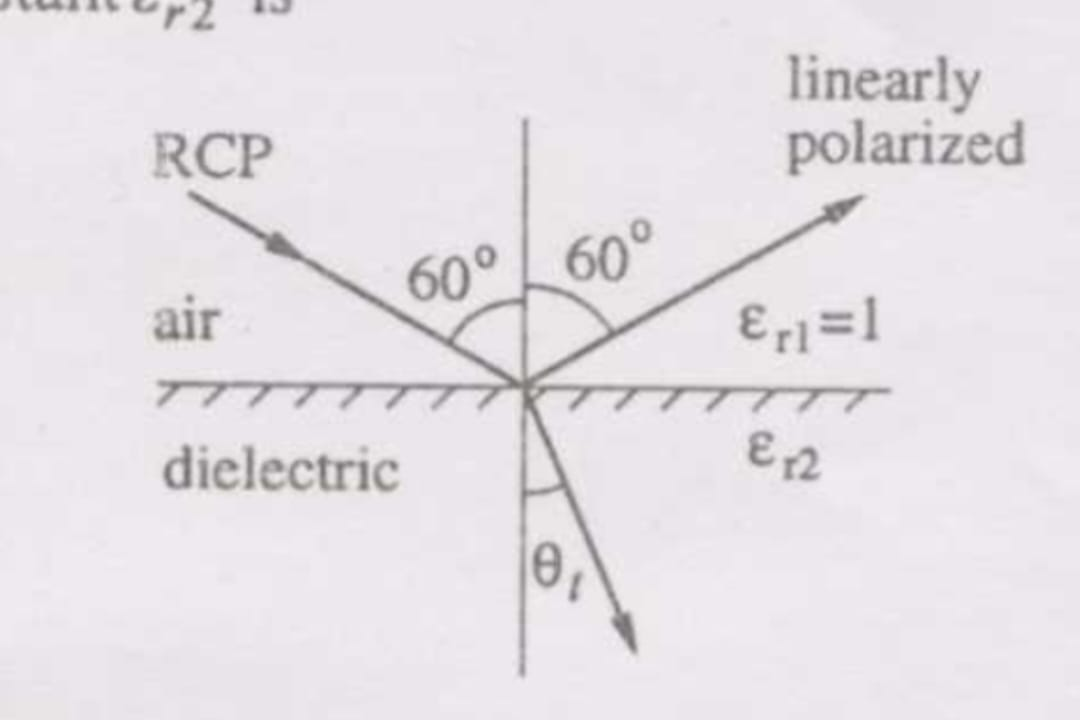
\includegraphics[width=0.4\textwidth]{Q70.jpg}
    \caption{}
    \label{fig:Q70.jpg}
\end{figure}

\hfill{\brak{\text{GATE EE 2025}}}

\begin{multicols}{4}
\begin{enumerate}
  \item $\sqrt{2}$
  \item $\sqrt{3}$
  \item $2$
  \item $3$
\end{enumerate}
\end{multicols}

{Common Data for Questions 71, 72, 73:} 
The figure shows high-frequency capacitance-voltage (CV) characteristics of a Metal/SiO$2$/silicon (MOS) capacitor having area $1\times10^{-4}\,\text{cm}^2$. Assume permittivities $\varepsilon_0$, $\varepsilon{\text{r}}$ of silicon and SiO$2$ as $1\times 10^{-12}\,\text{F/cm}$ and $3.5\times10^{-13}\,\text{F/cm}$ respectively. The measured capacitance transitions from $S\text{acc}$ (accumulation) to $S_\text{dep}$ (depletion/weak inversion) as gate voltage sweeps. A sketch:

\begin{figure}[ht!]
    \centering
    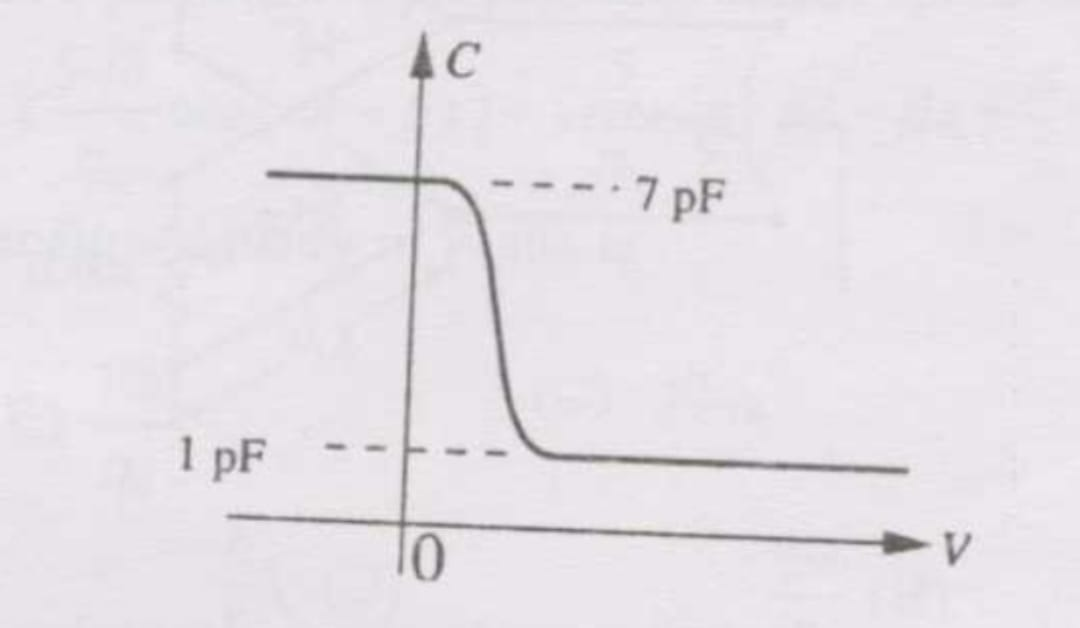
\includegraphics[width=0.5\textwidth]{Q71Q72Q73.jpg}
    \caption{}
    \label{fig:Q71Q72@73.jpg}
\end{figure}

\item The gate oxide thickness in the MOS capacitor is: 
\hfill{\brak{\text{GATE EE 2025}}}

\begin{multicols}{4}

\begin{enumerate}
  \item $50~\text{nm}$
  \item $143~\text{nm}$
  \item $350~\text{nm}$
  \item $1~\mu\text{m}$
\end{enumerate}
\end{multicols}

\item The maximum depletion layer width in silicon is:
\hfill{\brak{\text{GATE EE 2025}}}

\begin{multicols}{4}
\begin{enumerate}
  \item $0.143~\mu\text{m}$
  \item $0.857~\mu\text{m}$
  \item $1~\mu\text{m}$
  \item $1.143~\mu\text{m}$
\end{enumerate}
\end{multicols}

\item Consider the following statements about the CV characteristics plot:

S1: The MOS capacitor has an $n$-type substrate. \\
S2: If positive charges are introduced in the oxide, the CV plot will shift to the left. \\
Then which of the following is true?
\hfill{\brak{\text{GATE EE 2025}}}
\begin{enumerate}
  \item Both S1 and S2 are true
  \item S1 is true and S2 is false
  \item S1 is false and S2 is true
  \item Both S1 and S2 are false
\end{enumerate}


Common Data for Q.74 and Q.75: Two 4-ary signal constellations are shown. It is given that $\phi_1$ and $\phi_2$ constitute an orthonormal basis and four symbols in each are equiprobable. Let $N_0/2$ denote the power spectral density of white Gaussian noise. 

\begin{figure}[ht!]
    \centering
    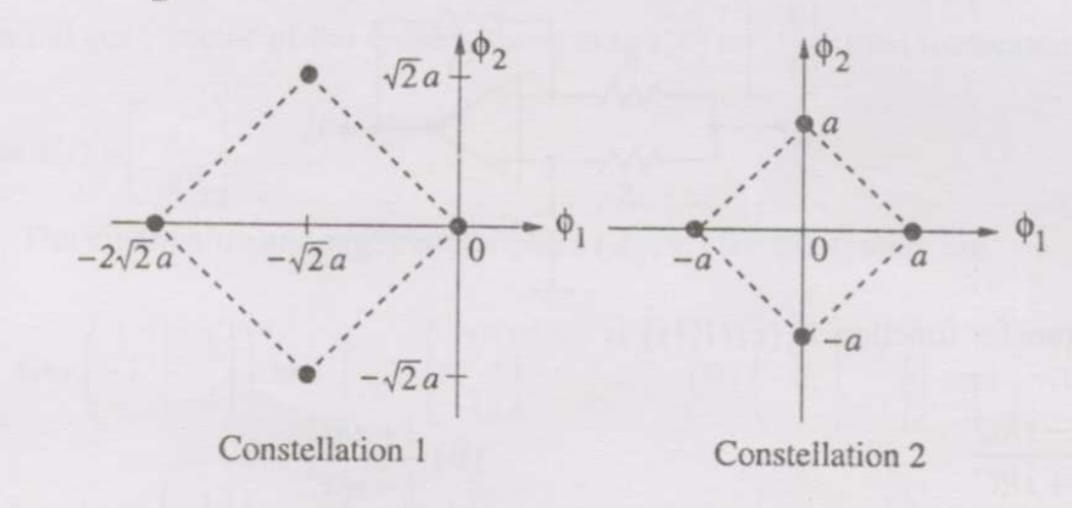
\includegraphics[width=0.6\textwidth]{Q74Q75.jpg}
    \caption{}
    \label{fig:Q74@75.jpg}
\end{figure}

\item The ratio of the average energy of Constellation 1 to that of Constellation 2 is:
\hfill{\brak{\text{GATE EE 2025}}}
\begin{multicols}{4}
\begin{enumerate}
  \item $4a^2$
  \item $4$
  \item $2$
  \item $8$
\end{enumerate}
\end{multicols}


\item If these constellations are used over an AWGN channel, then:
\hfill{\brak{\text{GATE EE 2025}}}
\begin{enumerate}
  \item Probability of symbol error for Constellation 1 is lower
  \item Probability of symbol error for Constellation 1 is higher
  \item Probability of symbol error is equal for both
  \item Value of $N_0$ will determine which has lower error
\end{enumerate}


Statement for Linked Answer Questions 76 \& 77: Consider the op-amp circuit shown. 

\begin{figure}[ht!]
    \centering
    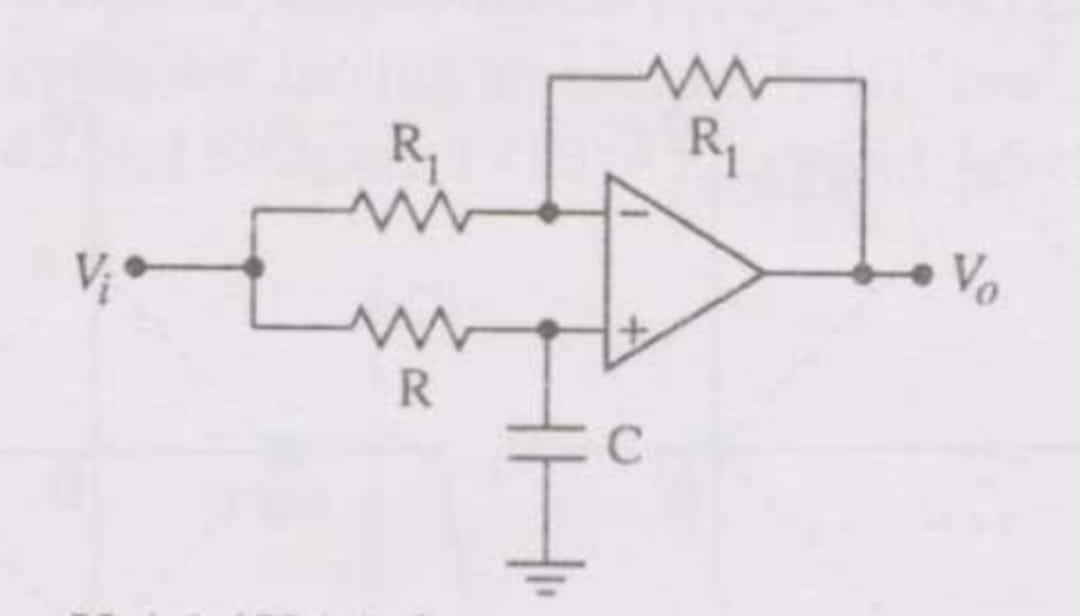
\includegraphics[width=0.4\textwidth]{Q76Q77.jpg}
    \caption{}
    \label{fig:Q76Q77.jpg}
\end{figure}

\item The transfer function $V_o(s)/V_i(s)$ is:
\hfill{\brak{\text{GATE EE 2025}}}
\begin{multicols}{4}
\begin{enumerate}
  \item $\dfrac{1-sRC}{1+sRC}$
  \item $\dfrac{1+sRC}{1-sRC}$
  \item $\dfrac{1}{1-sRC}$
  \item $\dfrac{1}{1+sRC}$
\end{enumerate}
\end{multicols}

\item If $V_i = V_i \sin(\omega t)$ and $V_o = V_o \sin(\omega t + \phi)$, the minimum and maximum values of $\phi$ (in radians) are respectively:
\hfill{\brak{\text{GATE EE 2025}}}
\begin{multicols}{4}
\begin{enumerate}
  \item $-\pi/2$ and $\pi/2$
  \item $0$ and $\pi/2$
  \item $-\pi$ and $0$
  \item $-\pi/2$ and $0$
\end{enumerate}
\end{multicols}

Statement for Linked Answer Questions 78 \& 79: An 8085 assembly language program is: 

\begin{verbatim}
1: MVI A, B5H
2: MVI B, 0EH
3: XRI 69H
4: ADD B
5: ANI 9BH
6: CPI 9FH
7: STA 3010H
8: HLT
\end{verbatim}


\item The contents of the accumulator just after execution of the \texttt{ADD} in line 4 will be:
\hfill{\brak{\text{GATE EE 2025}}}

\begin{multicols}{4}
\begin{enumerate}
  \item \texttt{C3H}
  \item \texttt{EAH}
  \item \texttt{DCH}
  \item \texttt{69H}
\end{enumerate}
\end{multicols}


\item After execution of line 7, the status of CY and Z flags will be:
\hfill{\brak{\text{GATE EE 2025}}}

\begin{enumerate}
  \item CY = 0, Z = 0
  \item CY = 0, Z = 1
  \item CY = 1, Z = 0
  \item CY = 1, Z = 1
\end{enumerate}

Statement for Linked Answer Questions 80 \& 81:

Consider a linear system whose state space representation is $\dot{x}(t) = A x(t)$.

If the initial state vector of the system is $\mathbf{x}(0) = \myvec{1  -2}$, then the system response is 

$\mathbf{x}(t) = \myvec{e^{-2t}  -2e^{-2t}}$. 

If the initial state vector of the system changes to $\mathbf{x}(0) = \myvec{1  -1}$,

then the system response becomes $\mathbf{x}(t) = \myvec{e^{-t}  -e^{-t}}$. [6pt]

\item The eigenvalue and eigenvector pairs $(\lambda, v)$ for the system are:  
\hfill{\brak{\text{GATE EE 2025}}}

\begin{enumerate}
  \item $\brak{-1,\quad \myvec{1 \\ -1}}$ \quad and \quad $\brak{-2,\quad \myvec{1 \\ -2}}$
  \item $\brak{-2,\quad \myvec{1 \\ -1}}$ \quad and \quad $\brak{-1,\quad \myvec{1 \\ -2}}$
  \item $\brak{-1,\quad \myvec{1 \\ -1}}$ \quad and \quad $\brak{2,\quad \myvec{1 \\ -2}}$
  \item $\brak{-2,\quad \myvec{1 \\ -1}}$ \quad and \quad $\brak{1,\quad \myvec{1 \\ -2}}$
\end{enumerate}
 
\item The system matrix $A$ is:  
\hfill{\brak{\text{GATE EE 2025}}}
\begin{multicols}{4}
\begin{enumerate}
  \item $\myvec{0 & 1 \\ -1 & 1}$
  \item $\myvec{1 & 1 \\ -1 & -2}$
  \item $\myvec{2 & 1 \\ -1 & -1}$
  \item $\myvec{0 & 1 \\ -2 & -3}$
\end{enumerate}
\end{multicols}

Statement for Linked Answer Questions 82 \& 83:

An input to a 6-level quantizer has PDF $f(x)$ as shown: it is piecewise-constant with three decision boundaries at $-1$, $0$, and $1$, chosen to maximize output entropy. The central plateau height is $a$, the outer flat region height is $b$. 

\begin{figure}[ht!]
    \centering
    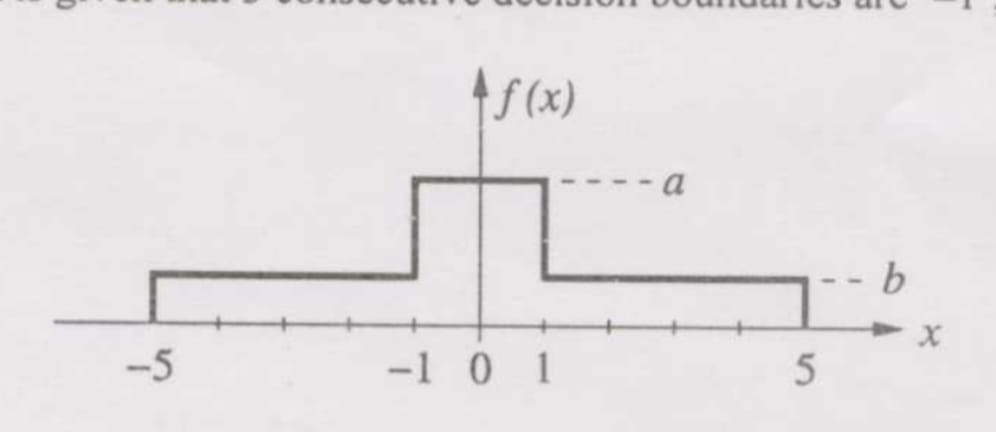
\includegraphics[width=0.4\textwidth]{Q82Q83.jpg}
    \caption{}
    \label{fig:Q82Q83.jpg}
\end{figure}

\item The values of $a$ and $b$ are:
\hfill{\brak{\text{GATE EE 2025}}}
\begin{multicols}{4}
\begin{enumerate}
  \item $a=\tfrac{1}{6},\ b=\tfrac{1}{12}$
  \item $a=\tfrac{1}{5},\ b=\tfrac{3}{40}$
  \item $a=\tfrac{1}{4},\ b=\tfrac{1}{16}$
  \item $a=\tfrac{1}{3},\ b=\tfrac{1}{24}$
\end{enumerate}
\end{multicols}

\item Assuming reconstruction levels are midpoints of decision intervals, the ratio of signal power to quantization noise power is:
\hfill{\brak{\text{GATE EE 2025}}}

\begin{multicols}{4}
\begin{enumerate}
  \item $\dfrac{152}{9}$
  \item $\dfrac{64}{3}$
  \item $\dfrac{76}{3}$
  \item $28$
\end{enumerate}
\end{multicols}

Statement for Linked Questions 84 \& 85:
In the DAC circuit shown, $V_R=10~\text{V}$ and $R=10~\text{k}\Omega$. The ladder consists of series $R$ sections with shunt $2R$ to ground, feeding an inverting op-amp with feedback resistor $R$. 

\begin{figure}[ht!]
    \centering
    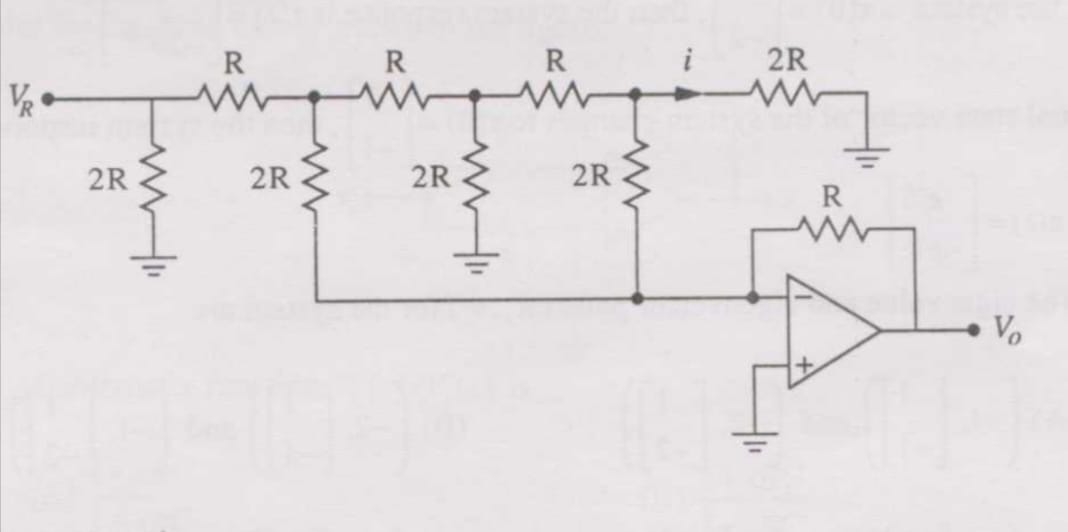
\includegraphics[width=0.5\textwidth]{Q84Q85.jpg}
    \caption{}
    \label{fig:Q84Q85.jpg}
\end{figure}

\item The current $i$ is:
\hfill{\brak{\text{GATE EE 2025}}}

\begin{multicols}{2}
\begin{enumerate}
  \item $31.25~\mu\text{A}$
  \item $62.5~\mu\text{A}$
  \item $125~\mu\text{A}$
  \item $250~\mu\text{A}$
\end{enumerate}
\end{multicols}

\item The output voltage $V_o$ is:
\hfill{\brak{\text{GATE EE 2025}}}

\begin{multicols}{2}
\begin{enumerate}
  \item $-0.781~\text{V}$
  \item $-1.562~\text{V}$
  \item $-3.125~\text{V}$
  \item $-6.250~\text{V}$
\end{enumerate}
\end{multicols}


\end{enumerate}

\end{document}

